\documentclass[a4paper,12pt]{article}

% Se vuoi che il pdf sia in formato mobile, decommenta la linea qui sotto e commenta la prima linea del codice
%\documentclass[1pt]{article}
\usepackage{enumitem}
\usepackage[paper size={90mm, 160mm},left=2mm,right=2mm,top=2mm,bottom=2mm,nohead]{geometry}
\usepackage{microtype}
\setlist[itemize]{leftmargin=*}


\usepackage{float}
\usepackage{url}
\usepackage{xcolor}
\usepackage{pdfpages}
\usepackage{graphicx}


%Comando per creare nuove definizioni stile blocco
\newcommand{\definition}[2]{
	\begin{table}[H]
	\centering
		\begin{tabular}{|p{0.9\linewidth}}
		\textbf{#1}\\ %Titolo della definzione
		#2\\%Testo della definizione
		\end{tabular}
	\end{table}
	\noindent
}

\newcommand{\df}[2]{\definition{#1}{#2}}

%%%%%%%%%%%%%%%%%%%%%%%%%%%%%%%%%%%%%%%%%%%%%%%%%%%%%%%%%%%%%%%%%%%%%
%      INSBOX --- macros for inserting pictures into paragraphs     %
%       Micha\l{} Gulczy\'nski, Szczecin, Jan 1996 / Feb 1998       %
%                     mgulcz@we.tuniv.szczecin.pl                   %
%%%%%%%%%%%%%%%%%%%%%%%%%%%%%%%%%%%%%%%%%%%%%%%%%%%%%%%%%%%%%%%%%%%%%
%
%  version 2.2
%
%  available macros:
%    * \InsertBoxC{anybox}
%        insert a centered box (use int _inside_ a paragraph)
%    * \InsertBoxL{after_line}{anybox}[correction]
%    * \InsertBoxR{after_line}{anybox}[correction]
%        insert a box in the left/right after specified number of lines;
%        correction specified in square brackets is optional;
%        both macros should be called _before_ a paragraph
%    * \MoveBelowBox
%        start a new paragraph just below the current frame
%
%  see the demo.tex file for more information
%

\catcode`\@ = 11
%
%  Margin between the text and the box:
\newdimen\@InsertBoxMargin
\@InsertBoxMargin = 2mm
%
%  definition of \ParShape, an inproved version of plain \parshape
%
\newcount\@numlines    % sum: m_1+...+m_n
\newcount\@linesleft   % counter used when reading lines of \ParShape
\def\ParShape{%
    \@numlines = 0
    \def\@parshapedata{ }% here we'll collect data for plain \parshape
    \afterassignment\@beginParShape
    \@linesleft
}%
\def\@beginParShape{%
    \ifnum \@linesleft = 0
      \let\@whatnext = \@endParShape
    \else
      \let\@whatnext = \@readnextline
    \fi
    \@whatnext
}%
\def\@endParShape{%
    \global\parshape = \@numlines \@parshapedata
}%
\def\@readnextline#1 #2 #3 {% #1 #2 #3 are: m_i, leftskip_i, rightskip_i
    \ifnum #1 > 0
      \bgroup  % I want to keep changes of \dimen0 and \count0 local
        \dimen0 = \hsize
        \advance \dimen0 by -#2  % \parshape requires left skip and
        \advance \dimen0 by -#3  % _length_of_line_ (not right skip!)
        \count0 = 0
        \loop
          \global\edef\@parshapedata{%
            \@parshapedata    % add to \@parshapedata:
            #2                % left skip
            \space            % a space
            \the\dimen0       % length of line
            \space            % another space
          }%
          \advance \count0 by 1
          \ifnum \count0 < #1
        \repeat
      \egroup
      \advance \@numlines by #1
    \fi
    \advance \@linesleft by -1
    \@beginParShape
}%
%
%  \InsertBoxC, \InsertBoxL, \InsertBoxR
%
\newbox\@boxcontent     % box containing the picture to be inserted
\newcount\@numnormal    % number of leading lines to typeset normally
\newdimen\@framewidth   % width of the frame
\newdimen\@wherebottom  % position of frame's bottom
\newif\if@byframe       % true if we are just beside the frame
\@byframefalse
%
%
\def\InsertBoxC#1{%
  \leavevmode
  \vadjust{
    \vskip \@InsertBoxMargin
    \hbox to \hsize{\hss#1\hss}
    \vskip \@InsertBoxMargin
  }%
}%
\def\InsertBoxL#1#2{%
  \@numnormal = #1
  \setbox\@boxcontent = \hbox{#2}%
  \let\@side = 0
  \futurelet \@optionalparameter \@InsertBox
}
\def\InsertBoxR#1#2{%
  \@numnormal = #1
  \setbox\@boxcontent = \hbox{#2}%
  \let\@side = 1
  \futurelet \@optionalparameter \@InsertBox
}%
\def\@InsertBox{%
  \ifx \@optionalparameter [
    \let\@whatnext = \@@InsertBoxCorrection
  \else
    \let\@whatnext = \@@InsertBoxNoCorrection
  \fi
  \@whatnext
}%
\def\@@InsertBoxCorrection[#1]{%
  \ifx \@side 0
    \@@InsertBox{#1}{0}{{\the\@framewidth} 0cm}%
  \else
    \@@InsertBox{#1}{1}{0cm {\the\@framewidth}}%
  \fi
}%
\def\@@InsertBoxNoCorrection{%
  \@@InsertBoxCorrection[0]%
}%
\def\@@InsertBox#1#2#3{%
  \MoveBelowBox
  \@byframetrue
  % \@wherebottom = \pagetotal + (\@numnormal * \baselineskip) +
  %                 (height of \@boxcontent) + (2 * \@InsertBoxMargin)
  \@wherebottom = \baselineskip
  \multiply \@wherebottom by \@numnormal
  \advance \@wherebottom by 2\@InsertBoxMargin
  \advance \@wherebottom by \ht\@boxcontent
  \advance \@wherebottom by \pagetotal
  % I have no idea why, but \InsertBox called at the top of a page
  % calculates space for the box one line too big
  \ifdim \pagetotal = 0cm
    \advance \@wherebottom by -\baselineskip  % ^ reduction
  \fi
  % add the correction
  \advance \@wherebottom by #1\baselineskip
  % \@framewidth = (width of \@boxcontent} + \@InsertboxMargin
  \@framewidth = \wd\@boxcontent
  \advance \@framewidth by \@InsertBoxMargin
  %
  \bgroup  % to keep changes of \dimen0 local
    % check if the box fits in the page
    \ifdim \pagetotal = 0cm
      \dimen0 = \vsize
    \else
      \dimen0 = \pagegoal
    \fi
    \ifdim \@wherebottom > \dimen0
      % print a warning message ...
      \immediate\write16{+--------------------------------------------------------------+}%
      \immediate\write16{| The box will not fit in the page. Please, re-edit your text. |}%
      \immediate\write16{+--------------------------------------------------------------+}%
      % ... and mark this place in document with a black box
      \vrule width \overfullrule
    \fi
  \egroup
  \prevgraf = 0
  % insert the box in the left (if #2 = 0) or in the right (if #2 = 1)
  \vbox to 0cm{%
    \dimen0 = \baselineskip
    \multiply \dimen0 by \@numnormal
    \advance \dimen0 by -\baselineskip
    \setbox0 = \hbox{y}%
    \vskip \dp0
    \vskip \dimen0
    \vskip \@InsertBoxMargin
    \ifnum #2 = 1
      \vtop{\noindent \hbox to \hsize{\hss \box\@boxcontent}}%
    \else
      \vtop{\noindent \box\@boxcontent}%
    \fi
    \vss
  }%
  % I have no idea why, but this is really necessary
  \vglue -\parskip
  \vskip -\baselineskip
  % each following paragraph needs to be formatted properly
  \everypar = {%
    % are we already below the bottom of the box?
    \ifdim \pagetotal < \@wherebottom
      % no...
      \bgroup  % to keep some changes local
        % let's calculate parameters for \ParShape
        \dimen0 = \@wherebottom
        \advance \dimen0 by -\pagetotal
        \divide \dimen0 by \baselineskip
        \count1 = \dimen0
        \advance \count1 by 1
        \advance \count1 by -\@numnormal
        \ifnum #2 = 1
          \ParShape = 3
                      {\the\@numnormal}   0cm   0cm
                      {\the\count1}       0cm   {\the\@framewidth}
                      1                   0cm   0cm
        \else
          \ParShape = 3
                      {\the\@numnormal}   0cm                  0cm
                      {\the\count1}       {\the\@framewidth}   0cm
                      1                   0cm                  0cm
        \fi
      \egroup
    \else
      % yes!
      \@restore@    % it's time to end everything
    \fi
  }%
  % this definition isn't very necessary --- just in case the paragraph
  % following \InsertBoxL or \InsertBoxR has fewer lines that the
  % first argument of the macro
  \def\par{%
      \endgraf
      \global\advance \@numnormal by -\prevgraf
      \ifnum \@numnormal < 0
        \global\@numnormal = 0
      \fi
      \prevgraf = 0
  }%
}%
%
%  call this macro to move the current position just below the
%  current frame
%
\def\MoveBelowBox{%
  \par
  \if@byframe
    \global\advance \@wherebottom by -\pagetotal
    \ifdim \@wherebottom > 0cm
      \vskip \@wherebottom
    \fi
    \@restore@
  \fi
}%
%
%  normal settings are as follows:
%
\def\@restore@{%
    \global\@wherebottom = 0cm
    \global\@byframefalse
    \global\everypar = {}%
    \global\let \par = \endgraf
    \global\parshape = 1 0cm \hsize
}%
%
%  someone told me that in LaTeX there is no \pageno counter;
%  the counterpart is \c@page
%
\ifx \documentclass \@Dont@Know@What@It@Is@
\else
  \let \pageno = \c@page
\fi


\catcode`\@ = 12

\newcommand{\lessonDate}[1]{\InsertBoxR{0}{\tiny{#1}}}

\newcommand{\E}{\`E\space}

\usepackage{listings}
\lstset{language=C++,
                keywordstyle=\color{blue},
                stringstyle=\color{red},
                commentstyle=\color{green},
                morecomment=[l][\color{magenta}]{\#}
}

\sloppy
\begin{document}

\begin{titlepage}
\begin{center}
	\Large{\textbf{Appunti di Sicurezza Informatica}}
\vfill
\normalsize{Caccaro Sebastiano}\\
\normalsize{A.A.2019/2020}
\end{center}
\end{titlepage}

\tableofcontents

\clearpage


%Lezione di 10 Ottobre 2019
\lessonDate{10 Ottobre 2019}
\section{Introduzione}
\textbf{Sito del corso}: \url{http://security.di.unimi.it/sicurezza1920/sec2.shtmls}\\
L'esame sarà a febbraio\\
\textbf{Modalità esame}: parte a quiz fatta computer + parte pratica sempre fatta a computer.

\section{Memory Errors}
Specialmente in certi linguaggi di programmazione, come C e C++, che non hanno meccanismi di controllo su quello che fa il programmatore con la memoria. Posso quindi sovrascrivere zone di memoria che non sono di mia competenza. Posso quindi creare degli \textbf{unexpected behaviour}.\\
Posso usare queste falle per comportamenti malevoli, come eseguire codice scritto da un attaccante ecc, per rubare dati ecc.\\
Sono scritti in C o C++ componenti che devono essere velocissimi, come sistemi operativi e sistemi critici, server web, embedded sistems.\\
Altri linguaggi non hanno questi problemi perchè inseriscono dei controlli, ma a scapito delle perfomance.

\subsection{Buffer Overflow}
\subsubsection{Storia}
Comincia del 1988 con il \textbf{Morris Worm}. Nel giro di 3-4 ore butta giù tutta la DarpaNet, prendendo una multa di 10-100 milioni di dollari, galera ecc.
\definition{Worm}{Programma che si autoreplica e si diffonde in varie macchine}
Nel 2001 \textbf{Code Red} infetta 300.000 macchine in 14 ore, nel 2003 \textbf{SQL Slammer} infetta 75.000 macchine in 10 minuti.\\
Molte vulnerabilità non vengono mai corrette, perchè comunque l'applicazione funziona lo stesso.
\subsubsection{Layout di memoria}
\definition{Memoria Virtuale}{Modalità di visualizzazione della memoria nella quale un processo vede tutta la memoria come se fosse assegnata solo a lui.}

\begin{figure}[H]
	\centering
	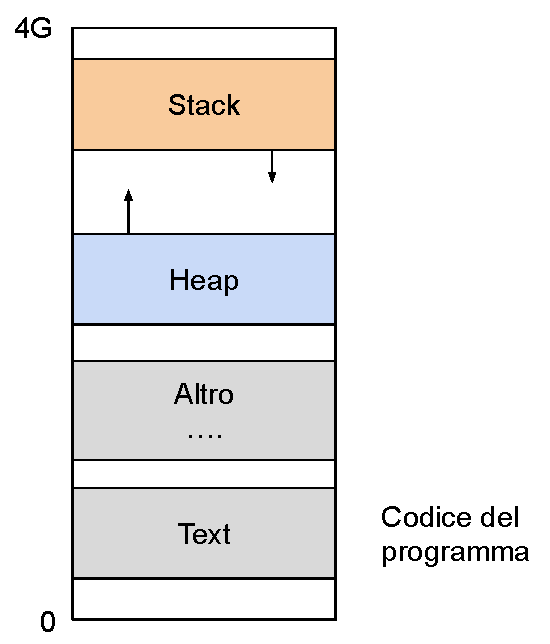
\includegraphics[width=0.5\linewidth]{Immagini/Stack1.pdf}
	\caption{Layout di memoria nei processori Intel}
\end{figure}

Mentre lo Stack cresce verso il basso, lo Heap cresce verso l'alto. Quindi, se nello stack per allocare devo sottrarre (andare giu), nello heap devo andare verso l'alto.\\
Lo Heap contiene perlopiù variabili allocate dal programmatore. Nello Heap, per allocare memoria, devo usare \texttt{malloc(sizeof(tipo))}. Una volta che non mi serve più quella zona, la libero con un \texttt{free}.

\subsubsection{Funzionamento dello Stack}

\begin{figure}[H]
	\centering
	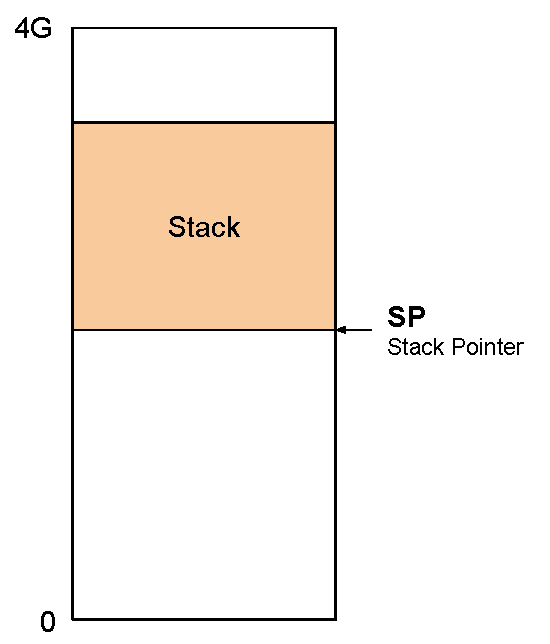
\includegraphics[width=0.5\linewidth]{Immagini/Stack2.pdf}
	\caption{Stack Pointer}
\end{figure}

Solitamente lo stack è utilizzato dal programma, in genere per le chiamate a funzioni. Lo stack è delimitato dallo \textbf{stack pointer}.

\begin{figure}[H]
\centering
\begin{lstlisting}[xleftmargin=.35\textwidth]
function(a1,b,c)
  int z
  strcpy(a,a1)
  return
  
main(...)
  function(a,b,c)
  Y:RET	
	
\end{lstlisting}
\caption{Esempio di chiamata a funzione}
\end{figure}

\begin{figure}[H]
	\centering
	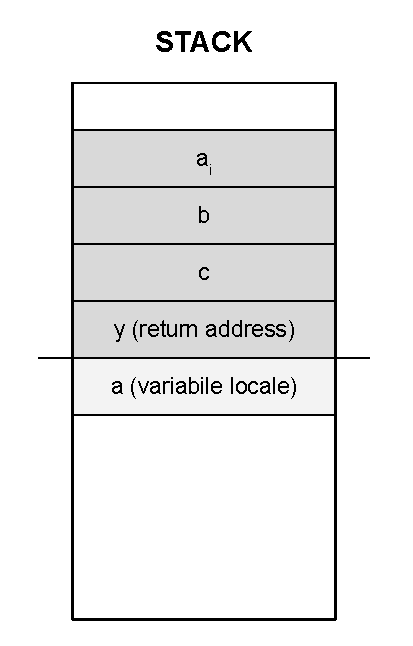
\includegraphics[width=0.4\linewidth]{Immagini/Stack3.pdf}
	\caption{Stack Pointer dell'esempio precedente}
\end{figure}

Quando vado ad eseguire la funzione, alloco anche un return address, che mi serve per capire dove andare alla fine della funzione. I parametri della funzione vengono poi espressi in funzione della posizione dello stack pointer (SP+16 bit ecc). Alla fine della funzione, sposto l'instruction a pointer viene impostato con il valore presente in Y, ovvero il return address. \E compito del chiamante poi togliere dallo stack gli altri parametri (\texttt{a}, \texttt{b} e \texttt{c}).
Cosa succede quindi ad una chiamata?\\
Chiamando la funzione:
\begin{enumerate}
\item Push degli argomenti nello stack
\item Push del return address
\item Jump all'indirizzo della funzione
\end{enumerate}
Tornando alla funzione principale:
\begin{enumerate}
\item Ritorno allo stack frame precedente
\item Torno al return address
\end{enumerate}

\subsubsection{Problematiche}
\definition{Buffer Overflow}{Operazione di scrittura che va a eccedere la locazione di memoria allocata a un dato dato.}

\begin{figure}[H]
\begin{lstlisting}[language=C++, xleftmargin=.3\textwidth]
void func(char *arg1)
{
 int authenticated = 0;
 char buffer[4];
 strcpy(buffer, arg1);
 if (authenticated) {...
 ...
}

int main()
{
 char *mystr = "AuthMe!";
 func(mystr);
 ...
}
\end{lstlisting}
\caption{Programma che esegue un buffer overflow}
\end{figure}

\begin{figure}[H]
	\centering
	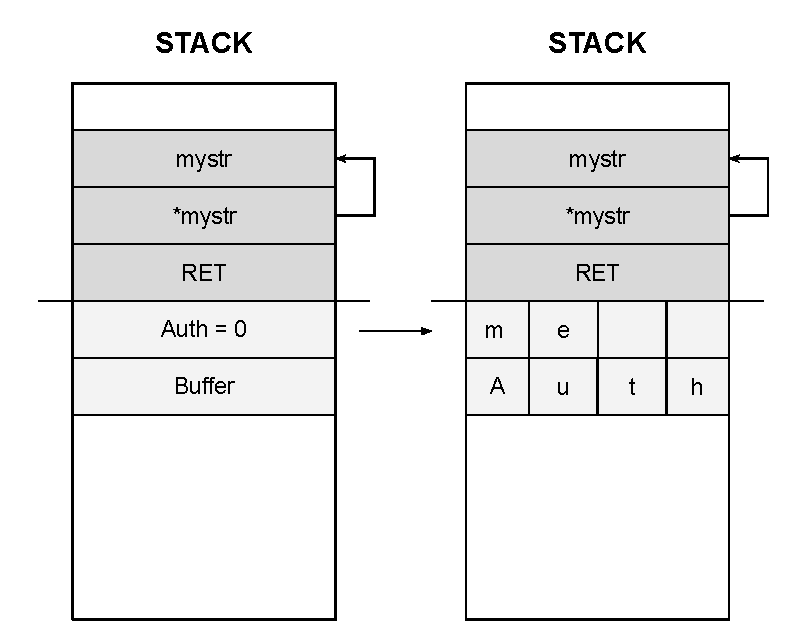
\includegraphics[width=0.8\linewidth]{Immagini/Stack4.pdf}
	\caption{Stack dell'esempio precedente}
\end{figure}
Sto provando a copiare una stringa "\texttt{AuthMe}" nel buffer a 4 byte. Siccome un carattere corrisponde a un byte, riesco a copiare solamente "\texttt{Auth}". Quindi, per scrivere il "\texttt{Me}" devo andare sopra nello stack. Quindi ho scritto "\texttt{Me}" nella variabile \texttt{Authenticated}, che adesso è diversa da 0. Ora quindi sono autenticato!\\
Con questo metodod potrei tranquillamente sovrascrivere tutto lo stack. Potrei, ad esempio, \textbf{sovrascrivere il return address}, saltando quindi in qualsiasi punto all'interno del programma, addirittura a parti del codice inserite in modo malevolo.

\subsubsection{Code Injection}
Lo scopo di una \textbf{Code Injection} è quello di fornire il codice da eseguire all'interno del programma. Purtroppo non posso metterla all'interno della sezione \texttt{Text}, perchè è read-only. Mettiamo quindi il codice all'interno dello stack.

\begin{figure}[H]
\begin{lstlisting}[language=C++, , xleftmargin=.3\textwidth]
void func(char *arg1)
{
 char buffer[4];
 sprintf(buffer, arg1)
}
\end{lstlisting}
\caption{Snippet}
\end{figure}
L'idea è quella di sovrascrivere buffer fino al return address. Il mio scopo è quello di inserire il mio codice all'interno di buffer, fino ad arrivare alla zona di memoria del return address. Nel return address andrò quindi a puntare l'indirizzo di memoria nel buffer, andando quindi ad eseguire il codice contento all'interno di essa.\\
Ma come faccio a sapere l'indirizzo di memoria attuale del buffer? Siccome la memoria è virtuale, riesco a sapere più o meno un range dove si trova l'indirizzo del buffer. Quindi inserisco prima del codice una sequenza di \textbf{\texttt{NOP}}, una cosidetta \textbf{NOP-sled} (pista d'atterraggio) per il mio codice.
\definition{NOP}{Short for NO Operation. Istruzione assembly che dice al processore di non fare niente per un ciclo di clock}

Devo quindi avere le seguenti cose:
\begin{itemize}
\item Distanza da sovrascrivere
\item Codice da inserire (inteso come codice macchina, binario, ancora più basso dell'assembly)
\item Indirzzo del buffer
\end{itemize}

Creo quindi il cosidetto \textbf{attack vector}.

\definition{Attack Vector}{Input che devo fornire al programma per inserire il mio exploit}

Per capire un po'meglio dove è il return address, provo a sovrascrivere con dati a caso sempre più grandi. Se il programma crasha, vuol dire che sta probabilmente cercando di saltare a un indirizzo a caso. Quindi è probabile che abbia trovato il return address.

\begin{figure}[H]
	\centering
	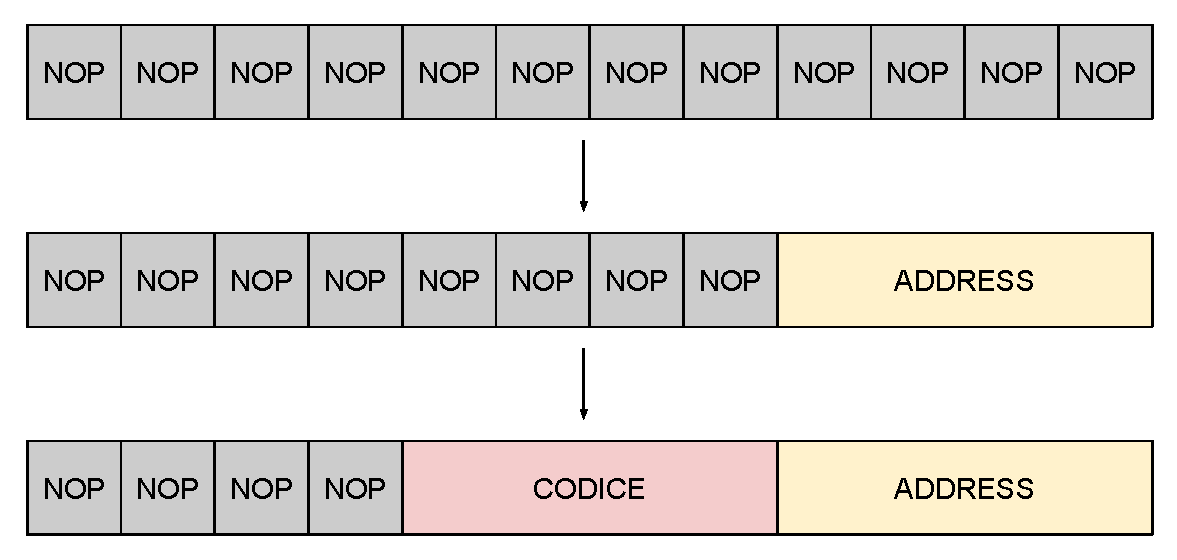
\includegraphics[width=0.8\linewidth]{Immagini/AttackV1.pdf}
	\caption{Costruzione di un attack vector}
\end{figure}

\begin{figure}[H]
	\centering
	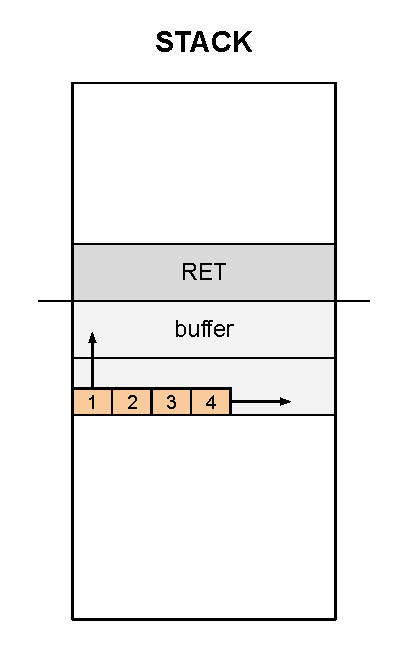
\includegraphics[width=0.4\linewidth]{Immagini/Stack5.pdf}
	\caption{Processo di scrittura della memoria}
\end{figure}
Il mio scopo solitamente è quello di acquisire maggiori privilegi. Lo faccio tramite qui programmi denominati \textbf{set whith rooot}, ovvero quei programmi che possono essere eseguiti da un utente normale ma che girano con permessi di root.

\subsubsection{Esempio di Code Injection}
Esercizio 1 disponibile qui \url{⎄https://github.com/andrealan/Software-Security-Lab/tree/master/bof-exercise}
\definition{Shell Code}{Codice che esegue una nuova finestra della shellS}
Il programma attaccante dichiara lo \textbf{shell code}. Nel main viene creato l'attack vector.
\begin{enumerate}
\item Creo un buffer
\item Lo riempio di NOP
\item Dichiaro l'offset rispetto al stack pointer, potrei doverlo cambiare
\item Inserisco il valore dell'indirizzo all'inizio
\item Scrivo lo shellcode dopo l'indirizzo
\end{enumerate}

\noindent\textbf{\Large IMPORTANTE}\\
 \textbf{La lettura nello stack avviene verso l'alto}. Quindi la NOP sled più che come una discesa, può essere pensata come un uno skilift.
 
\begin{figure}[H]
	\centering
	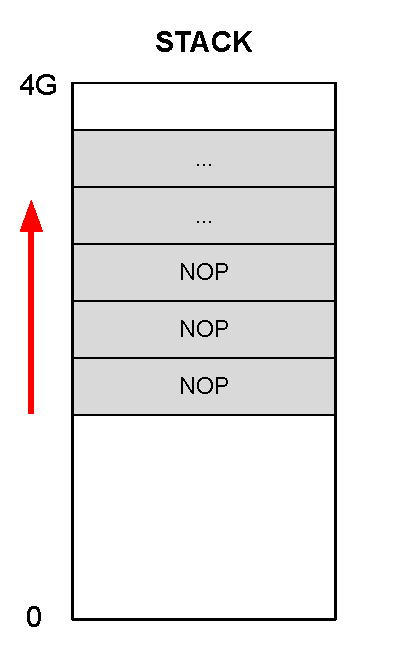
\includegraphics[width=0.4\linewidth]{Immagini/Stack6.pdf}
	\caption{La lettura dello stack avviene verso l'alto}
\end{figure}




\end{document}
